\section{DeepEMhancer Sharpening protocol}
\label{app:deepEMhancerSharpening}%a062

Protocol designed to apply $DeepEMhancer$, the automatic map postprocessing method that sharpens and masks part of the noise at medium/high resolution \citep{Sanchez-Garcia2020.06.12.148296}, in \scipion. Detailed information of this method can be also obtained in \url{https://github.com/rsanchezgarc/deepEMhancer}.

\begin{itemize}
 \item Requirements to run this protocol and visualize results:
    \begin{itemize}
        \item \scipion plugin: \ttt{scipion-em}
        \item \scipion plugin: \ttt{scipion-em-xmipp}
        \item \scipion plugin: \ttt{scipion-em-chimera}
    \end{itemize}
 \item \scipion menu:\\
  \ttt{Model building -> Preprocess map} (\ffigure{fig:app_deepEMhancer_1} (A))
  
 \item Protocol form parameters (\ffigure{fig:app_deepEMhancer_1} (B)):
  
    \begin{figure}[H]
     \centering 
     \captionsetup{width=.9\linewidth} 
     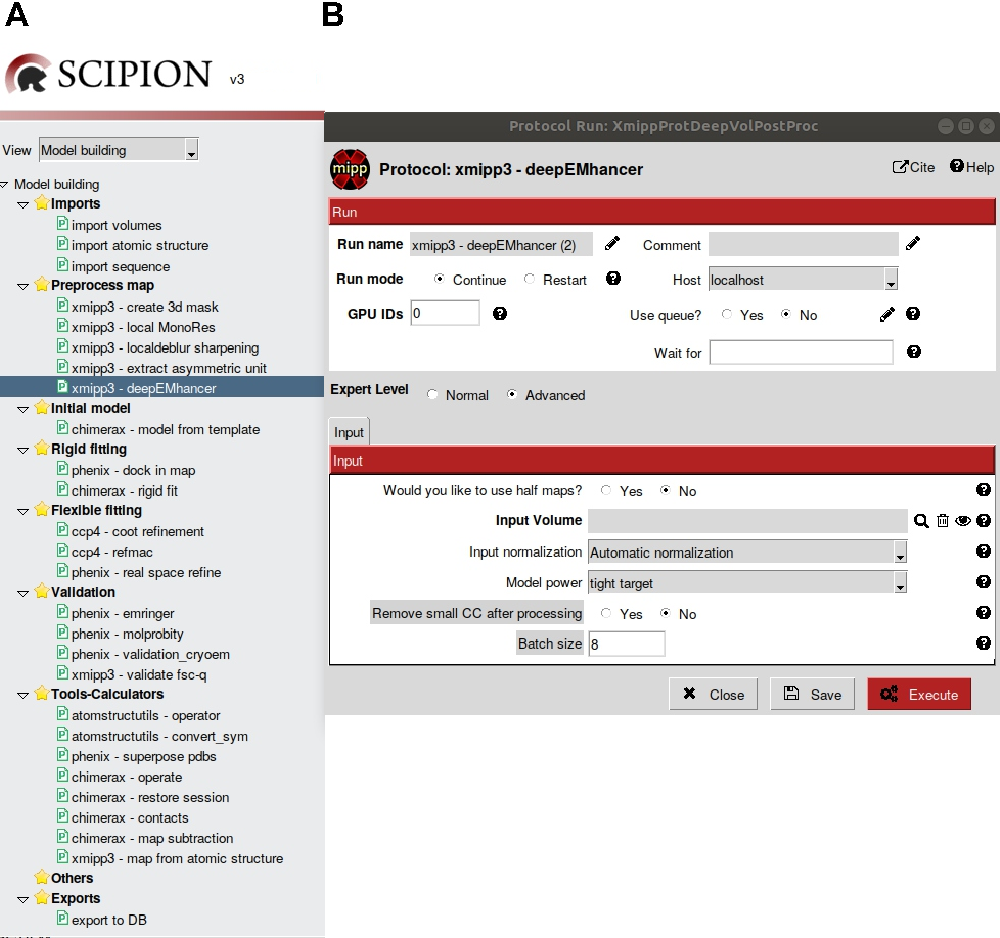
\includegraphics[width=0.90\textwidth]{Images_appendix/Fig303}
     \caption{Protocol \scommand{xmipp3 - deepEMhancer}. A: Protocol location in \scipion menu. B: Protocol form.}
     \label{fig:app_deepEMhancer_1}
    \end{figure}
    
    \begin{itemize}
        \item \ttt{Would you like to use half maps?}: Although the result will be the same if you decide to use half maps or a non-sharpened non-masked map, a way to ensure that you have selected the right input map is providing half maps. In addition, the algorithm has been trained with half maps. The first step performed by the protocol is to compute the average map. Then, select \ttt{Yes} whenever you can provide half maps, otherwise be sure you have the right average map, usually generated during the reconstruction process (after map refinement). However, the algorithm does not work correctly using post-processed maps. Since the two half maps can be obtained directly as independent maps or being associated to the average map, if you select \ttt{Yes} a new question will appear:
            \begin{itemize}
            \item \ttt{Are the half maps included in the volume?}: Select \ttt{Yes} if your input average map has the two half maps associated. If this is the case, complete the next form param. Otherwise, you should provide both half maps as independent preexisting \scipion objects. To add those half maps a couple of form params will apper to fill in with each half map:
                \begin{itemize}
                \item \ttt{Volume Half 1}
                \item \ttt{Volume Half 2}
                \end{itemize}
            \end{itemize}
        \item \ttt{Input Volume}: Unsharpened unmasked electron density map previously downloaded or generated in \scipion.
        \item \ttt{Input normalization}: We need apply normalization to accomodate the intensity values of the map to the specific range of values of the trained neural network. Three possible normalization methods are suggested:
        \begin{itemize}
            \item \ttt{Automatic normalization}: Default normalization mode that forces the noise average to be zero and the standard deviation 0.1 in an spheric shell around the specimen. Since then the noise always displays a similar distribution, the network gets easier to distinguish noise from signal. This method usually works correctly in almost any case. Exceptions could be very long specimens (fiber proteins) or those having big empty spaces (big viruses).
            \item \ttt{Normalization from statistics}: Similar to the first one, though in this case users provide their own statistics of the noise (average and standard deviation). Using $ChimeraX$ could be a good option to compute statistics of the noise such as min and max values, mean, standard deviation from the mean (SD) and root-mean-square deviation from zero (RMS) (command line \ttt{measure mapstats} with the option \ttt{subregion}; \url{https://www.cgl.ucsf.edu/chimerax/docs/user/commands/measure.html#mapstats}).   
            \item \ttt{Normalization from binary mask}: Select this option only if your input map is a masked map, which otherwise is not recomendable when this algorithm is used. The binary mask assigns 1 to the specimen and 0 to the remaining density.
        \end{itemize}
        \item \ttt{Model power}: Deep learning model to use, three options are available:
         \begin{itemize}
            \item \ttt{tight target}: This default model is a equidistant balanced solution that works properly for maps that show resolution areas between 3.8 and 6  \AA  (wide range of resolution values).
            \item \ttt{highRes}: This model allows a deep sharpening and it is recommended for high resolution maps (lower than 4  \AA).\\
            (Note: In case your map shows a high heterogeneity with parts of high resolution, as well as areas of low resolution, using \ttt{tight target} and \ttt{highRes} is recommendable, studying which areas are better sharpened by each model).
            \item \ttt{wide target}: This is the most conservative model. It is recommended when you have areas in which signal and noise are almost identical. Whereas \ttt{tight target} and \ttt{highRes} might delete those regions considering them only noise, \ttt{wide target} will surely preserve them.
         \end{itemize}
        \item \ttt{Remove small CC after processing}: Advanced param that improves the sharpening result by removing small connected components (usually noise). The default value of this param is \ttt{No} because the improvement usually does not make up for the additional time and computational resources invested.
        \item \ttt{Batch size}: Since $DeepEMhancer$ processes maps by dividing them in portions or smaller cubes that will be sent to GPUs, the value of batch size indicates the number of cubes that GPUs can simoultaneously process. Increase or reduce the default number according to the performance of the GPUs.
    \end{itemize}
    
    \item Protocol execution:\\
  Adding specific map/structure label is recommended in \ttt{Run name} section, at the form top. To add the label, open the protocol form, press the pencil symbol at the right side of \ttt{Run name} box, complete the label in the new opened window, press OK and, finally, close the protocol. This label will be shown in the output summary content (see below). If you want to run again this protocol, do not forget to set to \ttt{Restart} the \ttt{Run mode}.\\
  (Remark: In this case you have the option \ttt{GPU IDs} that you have to complete according to your GPU core indexes.)
  Press the \ttt{Execute} red button at the form bottom.
  
  \item Visualization of protocol results:
  
  After executing the protocol, press \ttt{Analyze Results} and \chimera graphics window will be opened by default. Both the input map(s) and the sharpened map generated by $DeepEMhancer$ (\ttt{deepPostProcess.mrc}) are referred to the origin of coordinates in \chimera. To show the relative position of atomic structure and electron density volume, the three coordinate axes are represented; X axis (red), Y axis (yellow), and Z axis (blue). Coordinate axes, input volume, and sharpened map are model numbers \ttt{\#1}, \ttt{\#2} , and \ttt{\#3}, respectively, in \chimera \ttt{Model Panel}. In case that half maps have been included, the respective additional model numbers will be applied.\\
  
  The possibility of visualizing the sharpened map by slices with $ShowJ$ (\url{https://github.com/I2PC/scipion/wiki/ShowJ}) is also open as commonly in \scipion, selecting in the \ttt{Output} of the \ttt{Summary} box, black arrow \ttt{xmipp3 - deepEMhancer -> Volume}, the right mouse option \ttt{Open with DataViewer}. 
  
  \item Summary content:
  \begin{itemize}
     \item Protocol output (below \scipion framework):\\ \ttt{xmipp3 - deepEMhancer -> Volume};\\ Volume (x, y, and z dimensions, sampling rate).
     \item \ttt{SUMMARY} box:\\ \ttt{Input}: type of map\\ \ttt{Normalization}: normalization method.
  \end{itemize}
    
\end{itemize}

